\section{Rump Kernel Ecosystem}
\label{chap:ecosystem}

In the previous chapters we examined the core architectures of the
anykernel and rump kernels.  In this chapter, we will look at
more practical aspects: how to build rump kernels on/for practically any
architecture/OS, how to link rump kernels into software stacks and
how to use the resulting software stacks.  In other words, this chapter
presents some use cases for rump kernels.  As opposed to the previous
chapter, we no longer limit the discussion to running rump kernels in
NetBSD userspace.

We discuss software available from
\url{http://repo.rumpkernel.org}.


\subsection{buildrump.sh}

To be able to run software, one must first compile software.  Compiling
software is done through a build framework, at least for any non-trivial
project consisting of more than a handful of source modules.  The rump
kernel implementation grew around the native build framework of NetBSD.
When building rump kernels for userspace as part of a NetBSD-targeted
build, the right tools are automatically present and properly configured.
Those tools are not automatically present in other situations, especially
on non-NetBSD build hosts.  The \texttt{buildrump.sh} script addresses
the need of building rump kernel components on practically any POSIX-like
host.  The possible target platforms are legion.

At the core of \texttt{buildrump.sh} is NetBSD's intrinsic ability to
cross-build itself on any platform.  The build involves first building
the build tools as host binaries, and then moving on to build the
rump kernel binaries for the target system.  The cross-build is accomplished by a script
called \texttt{build.sh}~\cite{mewburn:build.sh}.  After a fashion,
the naming of \texttt{buildrump.sh} pays homage to the underlying script.

The script is available from
\url{http://repo.rumpkernel.org/buildrump.sh}, along with related
subroutine scripts.


\subsubsection{The Double-crossing Toolchain}
\label{sect:buildrump-toolchain}

Let us first consider what cross-building is.  A cross-build can be
from one OS or version to another, from one machine architecture to another,
neither, or both.  \texttt{buildrump.sh} always assumes the case of both,
which means for example that it will not perform probes which require
executing the target code.

The common case for the build host is an x86 Linux and the target is
building rump kernel components for x86.  In other words, in the common
case we are building from one OS to another, but are building for the same
machine architecture as the host.  Therefore, the host's compiler
knows how to generate target binaries.  We will use this knowledge to
optimize the user experience in the common case, while still supporting
other cases as well.

The typical approach to cross-building is to first obtain a
cross-toolchain and only after that proceed with the build.  Contrary to
standard practice, \texttt{buildrump.sh} does not build a toolchain.
Instead, it creates wrappers around a user-supplied toolchain and
builds the target binaries using those wrappers.  The wrappers make the
user-supplied toolchain look like a NetBSD toolchain, so that the NetBSD
Makefiles work.  For example, most compilers do not recognize the option
\texttt{-cxx-isystem}.  If the wrapper detects a compiler where that
option is not supported, the option is translated to \texttt{-isystem}
before the compiler is run.

The rationale behind using wrappers is convenience.  First, downloading
and building a cross-toolchain takes several times longer than building
the actual rump kernel components.  Second, since in the most common case
(and a few others) there already is a usable toolchain sans wrappers,
we would unnecessarily be burdening the user if we always required
a NetBSD-targeting toolchain.

In cases where there is no
possibility to use the host's toolchain, \eg when on Mac~OS~X which
uses a different object format (MACH-O vs. ELF), the user must obtain
a suitable toolchain before running \texttt{buildrump.sh}.  The
same requirement for first having to obtain a suitable toolchain also
applies when compiling to a different machine architecture, \eg to
ARM from an x86 host.

Some compilers may generate code for different machine architectures
based on the supplied flags.  For example, gcc targeting \textit{x86\_64}
will generate code for 32bit x86 if \verb+-m32+ is passed as
an argument.  As part of its output, \texttt{buildrump.sh} will publish
the wrappers which include the toolchain flags passed to
\texttt{buildrump.sh}.  So, for example, if an \textit{x86\_64} toolchain
and \verb+-m32+ is passed to \texttt{buildrump.sh},
a \verb+i386--netbsdelf+ toolchain will be generated by
\texttt{buildrump.sh}.  In Section~\ref{sect:rumprun} we will look at
how this set of wrappers can be used for further constructs on top of
rump kernels.


\subsubsection{POSIX Host Hypercalls}

The first use case of \texttt{buildrump.sh} was to make building the
rump kernel for Linux userspace practical and user-friendly.  For
the result to also be functional, a hypercall implementation
was required.  Due to that historical reason, the default mode of
operation of \texttt{buildrump.sh} is to also build the POSIX hypercall
implementation from \texttt{src-netbsd/lib/librumpuser} and also a handful
of other libraries and utilities such as \texttt{src-netbsd/lib/librumphijack}
and \verb+src-netbsd/usr.bin/rump_server+.

Different POSIX'y platforms have subtle differences, for example in
which POSIX version they conform to, and therefore what the exact set
of supported interfaces is.
The first phase of building with a POSIX platform as the target runs
a probe.  The probe is a normal GNU autoconfigure script which is hosted
in \texttt{src-netbsd/lib/librumpuser/configure}.  The configure script
checks for example if \verb+clock_nanosleep()+ is available, and therefore
if it can be used to accurately implement \verb+rumpuser_clock_sleep()+
or if a best-effort use of \verb+nanosleep()+ is all that is possible.

When not building for a POSIX platform, the POSIX hypercall build must
be explicitly disabled by the user.  Disabling the POSIX hypercall build
also disables the associated probe.


\subsubsection{Full Userspace Build}

Though the original purpose of \texttt{buildrump.sh} was to build
kernel components, especially after work on the Rumprun unikernel
(Section~\ref{sect:rumprun}) began, it became clear that some easily
invoked method for
producing the corresponding NetBSD kernel and userspace headers and core
userspace libraries, \eg libc and libm, was required.  This functionality
was bolted on to \texttt{buildrump.sh}, and can optionally be invoked.
It is worth taking the time to understand that producing full headers and libraries
is orthogonal to building to run \textit{on} a userspace platform.


\subsubsection{src-netbsd}
\label{sect:srcnetbsd}

To build rump kernel components, \texttt{buildrump.sh} needs the source code for
the relevant parts of the NetBSD tree.  Theoretically, any vintage of the
NetBSD source tree would work.  However, in practice, a new enough vintage
of the NetBSD tree is required.  Historically, the user was required to
obtain the NetBSD source tree before running \texttt{buildrump.sh}.  Since the
full NetBSD tree is large and since a majority of the tree is not relevant
for rump kernels, the relevant parts of the tree are now mirrored at
\url{http://repo.rumpkernel.org/src-netbsd}.  This source tree represents a
known-good and tested vintage of the NetBSD source tree for use with
rump kernels; the contents are a regularly updated snapshot of the
NetBSD development head.  The \texttt{checkout.sh} script in the
buildrump.sh repository handles the details of the mirroring process.

The src-netbsd repository supplies several branches, with the idea
being that the user can choose the minimal set of sources required for
their particular application.  The branches are listed
in Table~\ref{tab:srcnetbsd}.  These branches may be used
as either a submodule, or fully duplicated into third party
repositories.

\begin{table}[t]
\begin{tabular}{|l|p{11cm}|}
\hline
branch name & description \\
\hline
\hline
kernel-src & bare minimum sources necessary for building rump kernels.
	In addition to the kernel sources, the tools required for building
	rump kernels are also included in this branch. \\
\hline
user-src & various userspace libraries and utilities useful for common
	rump kernel applications, \eg \texttt{libm} and \texttt{ifconfig} \\
\hline
posix-src & rumpuser implementation for POSIX platforms \\
\hline
\hline
buildrump-src & kernel + posix, \ie what \texttt{buildrump.sh} builds by default \\
\hline
appstack-src & kernel + user, useful for \eg
	unikernels (Section~\ref{sect:rumprun}) \\
\hline
all-src & kernel + posix + user \\
\hline
\end{tabular}
\caption[src-netbsd branches]{
\textbf{src-netbsd branches}.  The first set of branches
are base branches which contain no overlap.  The second set of branches
are the convenience branches which contain a certain union of the
base branches.  You will most likely want to use a convenience branch
for your project.  The precise content lists for the base branches are
available from \texttt{src/sys/rump/listsrcdirs}.
}
\label{tab:srcnetbsd}
\end{table}


\subsection{Rumprun Unikernel}
\label{sect:rumprun}

The Rumprun unikernel is a unikernel~\cite{unikernel} OS framework built
on top of driver components provided by a rump kernels.  Essentially,
a unikernel is akin to an embedded system, where there is no separation
between the application and system components of the software stack.
Rump kernels are well-suited to building a unikernel
framework, since the OS side of a unikernel is composed almost exclusively
of drivers, as can be verified by examining the amount of non-driver
code in Rumprun.  While Rumprun is also applicable for bare metal embedded
systems, the trend towards the cloud and microservices has made Rumprun
particularly relevant due to the ability to run existing application-level
programs.

The general idea of a unikernel is to bundle the operating system side
components and application(s) into a single image.  When that image is
booted on a given platform, the instance is set up and the application
is run according to the specified configuration.
Notably, even though the application and system side components are
bundled into a single image, the concept is orthogonal to whether or
not both run in the same hardware protection domain.

The goal of Rumprun is to provide the simplest possible glue code for
rump kernels to realize the target.  We will discuss the inner
workings of Rumprun.  As usual, the exact details of how to build and
configure the image are left to the user documentation.

The scope of the Rumprun unikernel is to enable creating bootable
unikernel images from application-level source code.  Those images may
be manually launched to create instances.  Details on how to deploy and
manage a ``fleet'' of unikernel instances is beyond the scope
of Rumprun.  In other words, the \textit{Orchestrating System} for the
Rumprun unikernel is expected to be provided by 3rd parties.

As an option, Rumprun can provide a POSIX-like userspace environment
which allows turning unmodified POSIX programs into unikernel images.
An explicit goal of Rumprun was to enable existing POSIX'y code
to run with zero modifications.  That is not to say that everything will
work without modification --- consider that code occasionally must be
ported to run between regular Unix platforms --- rather that the ideal case
will not require code modifications.  Non-trivial applications and
libraries, \eg \textit{libcurl}, \textit{mpg123} and \textit{sqlite},
do work without any changes.  As we discuss Rumprun in this chapter,
we will point out some limitations in Rumprun to further illustrate when
code changes may be required.

A packaging system for tested and, where necessary, ported
POSIX'y code to run on Rumprun is available at
\url{http://repo.rumpkernel.org/rumprun-packages}.  Further discussion on
the packaging system is beyond the scope of this book.

The Rumprun unikernel works on top of x86 platforms on bare metal,
Xen~\cite{barham:xen}, KVM~\cite{kivity:kvm}, and others.  As of writing
this, there is also nascent ARM support and Rumprun has successfully
run networked services on an ARM evaluation board.  In the following
discussion, for machine dependent details, we will cover only x86,
and more specifically x86\_64.

Rumprun source code is available from
\url{http://repo.rumpkernel.org/rumprun}.  For an architecture diagram
of the software stack, refer to Figure~\ref{fig:rumprun-stack}.

\begin{figure}[t]
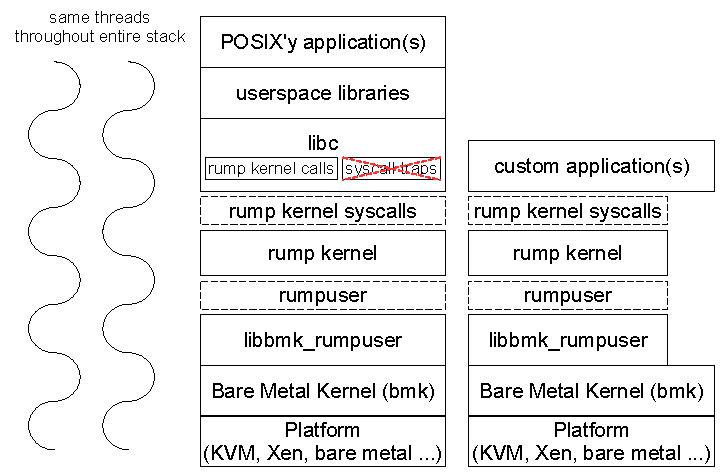
\includegraphics[width=\linewidth]{imgs/rumprun-stack}
\caption[Rumprun software stack]{\textbf{Rumprun software stack.}
Two modes are presented.  The one on the left includes the POSIX'y
userspace layers and can run unmodified programs.  The one on the
right is more lightweight, but mandates custom programs.  POSIX'y
programs are limited to POSIX'y interfaces, while custom applications
may call the underlying OS layer directly.  The specifics of
the layers are discussed throughout this chapter.
}
\label{fig:rumprun-stack}
\end{figure}

\subsubsection{bmk -- Bare Metal Kernel}

Since a rump kernel is not a real kernel, we need a real kernel in our
Rumprun software stack to provide functions which rump kernels do not give us.
For review, these functions include for example bootstrap, thread
creation, scheduling, interrupts and page level memory management.  We call
that kernel the \textit{Bare Metal Kernel}, or \textit{bmk} for short.
We will use the shorthand form from now on.  bmk was
originally written to demonstrate how to run rump kernels on
top of bare metal.  The more common recent use case is to run as a
virtualized service on top of \eg KVM, but the name stuck nonetheless.

The platform-specific implementations of bmk for Xen and non-Xen (e.g.
KVM and bare metal) are different in places.  We will limit our
discussion to non-Xen platforms.  The parts of the implementation
common to all platforms can be found under the source tree in
\verb+lib/libbmk_core+.  Platform-specific code is in
\texttt{platform/xen} and \texttt{platform/hw} for Xen and non-Xen,
respectively.


\subsubsection*{Bootstrap}

The first stages of bootstrap are beyond Rumprun and relegated to a
multiboot-compatible bootloader, provided by e.g. GRUB~\cite{grub} or
QEMU~\cite{qemu}.  The assembly entry point for bmk is at \verb+_start+
in \texttt{platform/hw/arch/amd64/locore.S}.  At the entry point, we save
information provided by multiboot (\eg memory size), set up bootstrap
pagetables, switch the CPU to 64bit mode --- a multiboot loader will
leave the CPU in 32bit mode --- set up the stack, and proceed to call
the C entry point \verb+x86_boot()+.  In other words, we do the minimum
of what more or less every operating system does at the early bootstrap
stage.

The C startup code initializes the console and performs various
architecture-specific initializations such as setting up the interrupt
controller.  Then, the scheduler is initialized, the page allocator is
set up, and finally the main thread is created by calling
\verb+bmk_sched_startmain()+.  The main thread eventually launches the
application.


\subsubsection*{Threads and Scheduling}

Recall, everything in a rump kernel runs in thread context
(Section~\ref{sect:procmodel}).
On Rumprun, everything except the lowest-level interrupt acknowledgement
runs in cooperatively scheduled thread context.
The scheduler, including thread creation and TLS support, is implemented in
\verb+lib/libbmk_core/sched.c+.  The Rumprun stack has no knowledge
of processes, apart from what rump kernels provide.

The rationale for cooperative scheduling is that it produces not only a
more readily repeatable result from one execution to another, but also ensures
that a thread is never preempted unless it has finished its work and
is ready to block.  In fact, a cooperative thread scheduler matches the
run-to-completion behavior of the rump kernel CPU scheduler.  Therefore,
the Rumprun unikernel will never encounter the situation where a host thread
is preempted with the rump kernel context held, and therefore unnecessary
host thread context switches are avoided.

In environments where the scheduler must protect against threads hogging
all CPU time and preventing other threads from running, cooperative
scheduling is not possible.  Since in a unikernel all threads are
essentially working towards the same goal, we can assume that there are no
hostile threads.  Of course, there is no reason why preemptive scheduling
could not be implemented for bmk, just that we have chosen not to do so.
Generally speaking, we are of the \textit{opinion} that cooperative scheduling
is more effective for the Rumprun unikernel, due to reasons mentioned
in the previous paragraph.

The rump kernel interacts with the scheduler via the hypercalls, as usual.
When a rump kernel hypercall encounters a situation where it decides to block,
it unschedules the rump kernel context, sets up the conditions for the
wakeup, and calls \verb+bmk_sched_block()+.  The scheduler then selects
the next thread to run, or if none are available, blocks and waits for
an interrupt to generate work.  Blocking via the rump kernel happens
completely transparently to POSIX-style applications using rump kernel
system calls.  Custom non-POSIX applications, in addition to blocking
via a rump kernel system call, may also call the bmk scheduler directly.
Figure~\ref{fig:bmkblock} illustrates with a stack trace how a POSIX
application interacts with the bmk scheduler.  In that particular case,
the wakeup will be generated by a timer interrupt; the timer interrupt
will wake the interrupt thread, which in turn will wake up the application
thread.

\begin{figure}[t]
{\tt \scriptsize
\begin{verbatim}
#0  bmk_sched_block ()                  [bmk]
#1  rumpuser_clock_sleep ()             [rumpuser]
#2  kpause ()                           [rump kernel]
#3  nanosleep1 ()                       [rump kernel]
#4  sys___nanosleep50 ()                [rump kernel]
#5  sy_call ()                          [rump kernel]
#6  sy_invoke ()                        [rump kernel]
#7  rump_syscall ()                     [rump kernel]
#8  rump___sysimpl_nanosleep50 ()       [rump kernel]
#9  __nanosleep50 ()                    [libpthread]
#10 _sleep ()                           [libc]
#11 main ()                             [application]
\end{verbatim}}
\caption[Rumprun stack trace for \texttt{sleep()}]
{\textbf{Rumprun stack trace for \texttt{sleep()}}.
The trace starts from the application and ends where bmk schedules
another thread.  The stack trace is annotated on the right with
descriptions of which logical component each stack frame belongs to.
}
\label{fig:bmkblock}
\end{figure}

The cooperative scheduling model exhibits a feature over the typical
preemptively scheduled pthreads.  Any program with a thread which runs
in a busy-loop without making blocking system calls will block the
entire system.  However, this type of behavior is not common and mostly
found in programs for scientific computation.  Nonetheless, one must be
aware of the limitation when choosing the programs which run on Rumprun.
If it is absolutely necessary to run such programs, the best option is
to insert yield calls into the busy-looping thread.  To ensure correct
execution of periodic tasks, application threads should yield or block
dozens of times per second.  Since yielding is cheap, it is better to
err on the side of doing it more often than necessarily.  Still, we want
to stress that in our experience, regular I/O bound programs ``just work''
without modification.


\subsubsection{Rumpuser}

The rumpuser hypercall interface for the rump kernel is
implemented on top of bmk.  The implementation resides in
\verb+rumprun/lib/lib/libbmk_rumpuser+.  The implementation can be used
as a reference implementation for rumpuser especially for cases with
underlying cooperative threading.  We leave perusing the implementation
to the interested reader.


\subsubsection{To Userspace (or Not To Userspace)}

As indicated in Figure~\ref{fig:rumprun-stack}, two modes of operation
are available: one which is capable of running POSIX'y userspace and one
which is not capable of that.
There are tradeoffs to including a full userspace stack in your unikernel
instance.  Throughout this text, by ``userspace'' we mean the normal
userspace environment available on a regular POSIX'y operating system.
On a unikernel, there is strictly speaking no hard division between
the kernel and userspace, but we nonetheless use the term ``userspace''
to describe the POSIX'y application portion of the stack.

Like on a regular operating system, the userspace environment is a
collection of library interfaces on top of which normal programs run.
The system call interface is an analogous, lower level set of interfaces, but
in most cases programs will run on top of the userspace environment,
not directly on system calls.  There are some exceptions, such as programs
written in Go~\cite{golang}, where the language runtime is implemented
directly on top of system calls.

The advantage of including userspace support is not only that POSIX
programs work out-of-the-box, but also that userspace interfaces are
mostly standard and stable.  Therefore, no matter the future work we
do on the Rumprun unikernel, we will always guarantee that
userspace interfaces remain stable.  We do not offer the same level
of guarantee for bmk, even if we attempt to minimize churn.

The disadvantage of the full userspace stack is its extra footprint.
Not only are userspace libraries mandated, but in practise the
rump kernel file system components are needed because of various
libc interfaces implicitly assuming the presence of certain
files, \eg \texttt{/etc/services} and \texttt{/etc/resolv.conf}.
Therefore, if you need to minimize your footprint, and you do not
have an existing, complex application written against POSIX interfaces,
you most likely want to avoid the userspace layers.


\subsubsection*{System Calls}

We know from Section~\ref{sect:syscallentry} that a rump kernel provides
ABI-identical system calls apart from a \verb+rump_sys_+ prefix in the
symbol name.  We also implicitly understand that some component in the
Rumprun software stack must provide the system calls under the same name
as a regular libc.  Furthermore, performing a system call must result
in the handler in the rump kernel being invoked.

The system call entry points in libc invoke the kernel via a hardware
trap.  Those entry points may be useful in the future if we wish to
run the application portion and system portion of the Rumprun stack in
separate protection domains.  However, in the simplest model we do not
wish to assume anything about the underlying platform's capability to
support privilege levels, and therefore the standard libc entry points
are not applicable.

\begin{figure}[t]
{\tt \scriptsize
\begin{verbatim}
#ifdef RUMP_KERNEL_IS_LIBC
__weak_alias(lseek,rump___sysimpl_lseek);
__weak_alias(_lseek,rump___sysimpl_lseek);
__strong_alias(_sys_lseek,rump___sysimpl_lseek);
#endif /* RUMP_KERNEL_IS_LIBC */
\end{verbatim}}
\caption[Userspace aliases for rump kernel syscalls]
{\textbf{Userspace aliases for rump kernel syscalls}.
Conditionally, a rump kernel can provide system calls with names that
a userspace environment expects.  Both user-visible overridable (weak)
and system-internal non-overridable (strong) aliases are provided.
Not all aliases are necessary for all system calls, but since they do
no harm, we provide them.  For discussion on the system call entry
point itself, see Section~\ref{sect:syscallentry}.  As usual,
there is a naming problem (with the macro name), but since the name
is not user-visible, it has not been worth the fuss to adjust the name.
}
\label{fig:rumpkernelislibc}
\end{figure}

We augment the rump kernel system call handlers to conditionally alias
the rump kernel entry point symbol to the libc symbols.  These aliases
are illustrated in Figure~\ref{fig:rumpkernelislibc}.  For the Rumprun
unikernel, we build the rump kernel with that conditional knob turned on.
Furthermore, we build libc without the usual trap-generating entry points.
When everything is linked together, an application unaware of rump kernels
calling \verb+foo()+ results in the same as an application aware of rump
kernels calling \verb+rump_sys_foo()+.  In effect, POSIX applications
on Rumprun act as local rump kernel clients without being aware of it.


\subsubsection*{POSIX Threads (pthreads)}

The POSIX threads or pthreads library offers a set of interfaces
upon which multithreaded applications can be realized.  Those
interfaces include for example ones for creating threads and performing
synchronization between threads.  Given the standard nature and widespread
use of pthreads, we wish to support programs which use pthreads.

Again, there are multiple straightforward ways on how to realize pthread
support.  One is to write a pthread library from scratch.  Another one
is to port a pthread library from another operating system.  However,
both of those approaches incur implementation effort and maintenance,
and are against our general principles of design.

We observe that the NetBSD pthread library is implemented 1:1 on top of
NetBSD's kernel threads, \ie the relation between an application pthread
and a kernel thread is a bijection.  To for example create a new thread,
libpthread uses the \verb+_lwp_create()+ system call, and to put the
current thread to sleep awaiting wakeup, \verb+_lwp_park()+ is called.

To support the NetBSD pthread library on top of the threads offered
by bmk, we implemented the \verb+_lwp+ interfaces against bmk in
\verb+lib/librumprun_base/_lwp.c+.  After that, we could use NetBSD's
libpthread to provide pthreads on Rumprun.

As an implementation detail, as of writing this, \verb+_lwp.c+
is implemented as libc-level symbols in the userspace package
(rumprun\_base).  Henceforth, software wanting to bypass libc and
use the lwp interfaces to implement their own threading, \eg the Go
runtime, must include userspace support.  This feature may be fixed at
a future date by pushing the implementation of the lwp interfaces into
the rump kernel.


\subsubsection*{Limitations}

Recall, rump kernels do not support virtual memory or preempting threads.
Therefore, rump kernels do not provide memory mapping (\texttt{mmap()},
\texttt{madvise()} and friends) or signals.  These two facilities are
used by some userspace applications.

For signals, we simply resort to stating ``signals are evil''.  (There are
advantages to this book no longer being an academic text.)  Therefore,
any application requiring signals for basic functionality will not work
without porting.  Coming up with mostly functional signal emulation,
where handlers are called at select points without preempting threads,
may be done at a future date.  Regardless of whether that will be emulated
or not, signals still are evil.

We emulate some aspects of memory mapping in the component
library located at \verb+lib/librumpkern_mman+.  Notably, emulation is
hooked in as rump kernel syscalls so that custom applications
may use that emulation.  Anonymous memory mapping is simply a
matter of allocating the right amount of memory, though Rumprun will not
respect the read/write/execute protection flags.  Memory mapping files
is more complicated, since the contents need to be paged in and out.
Since there is no virtual memory, there are no page faults, and contents
cannot be paged in on demand.  As of writing this, read-only mapping are
emulated by reading in the full contents at the time of the mapping.
While the approach is not perfect in many ways, it allows a decent set of
programs to work in some cases at the cost of a handful lines of code.


\subsubsection{Toolchain}

The Rumprun unikernel is always cross-compiled, which
means that the build process never runs on a Rumprun instance.  Instead,
the build process runs on a build host, \eg a regular Linux system.
To [cross-]build software, a toolchain is required.

For custom applications, we have no external standards to bow down
towards, nor do we want to impose any limitations on how to build
custom applications.  Therefore, it is up to the builder of the custom
application how to build and link the unikernel image.  A straightforward
way is to use the toolchain wrappers generated by \texttt{buildrump.sh}
(Section~\ref{sect:buildrump-toolchain}).  We will not further
discuss toolchains for custom applications.

For POSIX'y userspace applications, we do have external standards to bow down to.
Application are engineered to build using a build system (\eg GNU autotools or CMake).  Build systems assume that the toolchain
looks a certain way, and that the build consists of certain steps.
Those steps can be for example, probe, build and link.  Recall, in the best case
scenario unmodified applications work on a Rumprun unikernel.
It would be convenient if those applications could also be built for
the Rumprun unikernel without having to introduce changes to the build
system.  That was the goal of the application toolchain.  The rest of
the discussion in this section is on how that goal was accomplished.


\subsubsection*{The ABI}

When building application source code, one must decide which ABI to
build for.  That ABI will determine where the program can run.  Typically,
the ABI is signified by the \textit{tuple} ingrained into the toolchain.
For example, a \verb+x86_64-linux-gnu+ toolchain will produce a
binary which can run on an x86-64 machine with a Linux kernel and a GNU
userspace.  In other words, there is a machine architecture component
and a system side component to the ABI.  The binary can be run only on a
machine architecture and an operating system which supports the given ABI.
The obvious example of an operating system supporting the Linux-GNU ABI
is Linux, but it is also possible to other operating systems to emulate
various ABIs to allow running programs complied for a non-native ABI.

For Rumprun, we use the same tuple as NetBSD, \eg \verb+x86_64--netbsd+,
but insert ``rumprun'' into the otherwise empty vendor field.  Therefore,
for x86\_64 the ABI tuple of Rumprun is \verb+x86_64-rumprun-netbsd+.
The installed toolchain for building Rumprun images follows the standard
convention of naming binaries, \eg \verb+x86_64-rumprun-netbsd-ar+
and \verb+x86_64-rumprun-netbsd-gcc+.  Internally, the toolchain is a
set of wrappers around the toolchain provided by \texttt{buildrump.sh}, which in
turn is a set of wrappers around the toolchain supplied by the user.


\subsubsection*{The Implementation of the ABI}

In the normal case, the operating system implementing the system side
of the ABI is not bundled with the binary.  The operating system itself
comes to be when a certain selection of drivers implementing that ABI
is booted.  Notably, there is no strict contract between the ABI and
which drivers the operating system must provide for the program to
run correctly.  A Linux kernel without networking support can still run
Linux binaries, but programs using networking will not run as expected
on that particular Linux instance.

In other words, in the normal model, building \& booting the operating
system and building \& running applications are separate steps.  Normal build
systems also assume them to be separate steps, and do not include a step
to determine which operating system components should be linked into the
binary.  If we wish normal build systems to work without modification,
we must address this disparity on our side.


\subsubsection*{Pseudo-linking and Baking}

One solution for specifying the implementation of the ABI would be to hardcode
the set of rump kernel components into the toolchain and to identify the
set in the toolchain tuple.
However, that solution would mean creating a separate set of toolchain wrappers
for every desired component combination, and would be hard to manage.
Another option would be to always include all drivers, but it would be
wasteful, and also possibly would not work --- consider situations where
you have two mutually exclusive drivers for the same backend.

A more flexible solution comes from what we call \textit{pseudo-linking}.  When the
application part of the binary is linked, the operating system components
are not attached to the binary.  Instead, the application link phase
produces non-runnable intermediate format, which includes the objects
and libraries specified on the link command line.

The pseudo-link phase checks that all application symbol
dependencies are satisfied.  Again, doing so honors existing
conventions; this check is required for example by the
probe phase of some build frameworks, which determine if a certain
interface is supported by the given system by trying to link a test
program using that interface, and iff the link succeeds, mark that
interface as available.  It needs to be noted that these types of checks
apply only to userspace interfaces, and not to the kernel drivers backing
those interfaces, so things may still fail at runtime.  However,
limiting the check to userspace interfaces is what current POSIX'y
applications expect.

To produce the bootable unikernel image, the pseudo-linked intermediate
representation is \textit{baked}.  The baking process attaches the
operating system side driver components to the image, analogous to
the normal case where the operating system implementing the ABI is
booted.  Baking is done using the \verb+rumprun-bake+ tool.

The entire set of steps require for transforming source code to a bootable
unikernel image is illustrated in Figure~\ref{fig:rumprun-buildexample}.


\begin{figure}[t]
{\tt \scriptsize
\begin{verbatim}
$ cat > hello.c << EOF
> #include <stdio.h>
> int main() {printf("Hello, Rumprun!\n");}
> EOF
$ x86_64-rumprun-netbsd-gcc -c -o hello.o hello.c   # compile
$ x86_64-rumprun-netbsd-gcc -o hello hello.o        # pseudo-link
$ rumprun-bake hw_virtio hello.bin hello            # bake
\end{verbatim}}
\caption[Building a runnable Rumprun unikernel image]
{\textbf{Building a runnable Rumprun unikernel image}.
The different phases of the build are illustrated.  First, the object
files are compiled.  Second, the object files are pseudo-linked.
Any objects and libraries specified at this stage will be carried by
the intermediate representation.  Finally, the remainder of the Rumprun
stack is baked into the pseudo-linked intermediate representation.
In this example, we used the \textit{hw\_virtio} configuration,
which contains the I/O drivers for cloud hypervisors.  In case
\textit{hw\_generic} is specified instead, drivers for bare metal
would be included.
}
\label{fig:rumprun-buildexample}
\end{figure}

\subsubsection*{Pipelines and Multibaking}

Consider the Unix pipeline: a program generates output which is fed to the
next stage in the pipeline as input.  Therefore, a program does not need
the knowledge of how to generate the input or how to store the output,
as long as the program has the knowledge of how to process the data.
Assume we have such a program which knows how to process data, but not
whence the data is coming or where it is going to.  We wish to support
that concept in Rumprun, for example for cases where POSIX'y programs
are used as highly isolated data processors.

For example, imagine that the user wishes the main program to read input
using HTTP, but the program lacks intrinsic HTTP support.  This feat would
be accomplished on a regular system with \eg
``\verb+curl http://add.ress/input | prog+''.
There are a few possible routes to support the same in Rumprun.  We will
discuss some of those possibilities before discussing the option we chose.

\begin{itemize}
\item	\textbf{adjusting the main program}: our
	guiding principle throughout this entire work is to avoid
	unnecessary forking and modification.  In some cases teaching
	the main program may be necessary, for example when processing
	multiple small files is desired.  However, for this discussion
	we will consider adding knowledge of HTTP to the main program
	as a last resort.

\item	\textbf{use of a file system driver}: a file system is akin to
	a system-side pipeline, though possessing the additional features of
	named streams and seeking, among others.  It would be possible to
	hide the details of HTTP from an application inside a file
	system driver.	However, due to the above-mentioned additional
	features which are usually not not required in a pipeline, file
	system drivers require implementing a dozen-or-so methods to have
	even bare-bones functionality.  Therefore, the implementation
	effort of what could be accomplished with a handful of lines
	of application code is increased by at least an order of
	magnitude.
	%Granted, in the case of
	%HTTP, ready-made HTTP file system drivers exist on top of
	%FUSE~\cite{fuse}, but since those drivers are user-level programs,
	%we would again circle back to the original problem of wanting to
	%execute multiple application programs in a single Rumprun instance.
\end{itemize}

To solve the pipeline problem, we observe that a rump kernel already
supports multiple processes, as required by remote client support
(Section~\ref{sect:distributed}), and pipes between those processes
(\verb+rump_sys_pipe()+).
Using a regular pipe between the rump kernel processes allows data to
flow between the programs.  The remaining puzzle pieces come from the
separation of pseudo-linking and baking.  We allow \verb+rumprun-bake+
to take multiple binaries which are baked into the final executable.
For example, the following command will include both the processor and
transporter in the final runnable binary:

\begin{verbatim}
$ rumprun-bake hw_virtio rumprun.bin processor transporter
\end{verbatim}

This unikernel can then be run so as to imitate the following pipeline:

\begin{verbatim}
$ ./transporter r src | ./processor - | ./transporter w dst
\end{verbatim}

Note, in the current implementation the transporter and processor
share for example the same libc state and symbol namespace.  Therefore,
as of writing this, multibaking cannot be used to include multiple arbitrary
programs in the same Rumprun image.  However, the approach works in cases
where the transporter program is judiciously crafted to suit the purpose.
Support for arbitrary programs may or may not be added at a future date.


\subsubsection{PCI: Big Yellow Bus}
\label{sect:pci}

In Section~\ref{sect:usb} we looked at using USB devices in rump kernels.
Ignoring the desirability of that approach, for Rumprun the same approach
of relying on a thick underlying layer is not feasible --- the only
underlying software layer is bmk.  For Rumprun on x86 hardware(/KVM), the
desired peripheral I/O devices are on PCI busses.  To use those devices,
we provide PCI bus access via hypercalls, and use the PCI device drivers
provided by the rump kernel for actual device access.  The hypercalls
follow the boundaries of the MI/MD (machine in/dependent) code boundary
in NetBSD.  We stress that the discussion in this section is about x86
bare metal.

Essentially there are three classes of hypercalls that are required to
support PCI devices:

\begin{itemize}

\item	\textbf{PCI configuration space access}.  By accessing
	configuration space registers, software can determine which
	devices are present, alter PCI-specific behavior of the
	device, and gain access to the device-specific registers.
	Configuration space access is done using x86 I/O operations
	(\texttt{inl()}, \texttt{outl()}).  While those instructions
	could be used within the rump kernel without resorting to
	hypercalls, we use hypercalls for the benefit of being able
	to share the PCI code with other platforms which are not
	described here.

\item	\textbf{Interrupt handling}.  Establishing an interrupt
	means that when an interrupt is triggered on the CPU,
	the corresponding interrupt handler gets called to inspect
	the device.  While the process is simple in theory, a problem
	arises from mapping the device's idea of an interrupt line to the
	corresponding line detected by the CPU.  Most systems attempt to
	establish this relationship by parsing the relevant ACPI tables.
	We take a simplistic approach which does not require thousands
	of lines of code: since there are typically only 1-2 PCI I/O
	devices on a given Rumprun instance, we assume that all devices
	share an interrupt and call all handlers when any PCI interrupt
	arrives.  We may include proper support for interrupt routing
	at a future date, if a need arises.

\item	\textbf{DMA-safe memory handling}.  DMA is not a PCI-specific
	construct, but since PCI devices are the only devices on Rumprun
	which do DMA, we discuss DMA here.  Essentially, DMA is a matter
	of being able to allocate ``DMA-safe'' memory.  In practice,
	safety means physically contiguous memory which is allocated
	according to certain boundary and alignment constraints.
	The boundary constraint means the range must not cross a certain
	multiple, and alignment means that the range must start from
	the multiple.  Since bmk uses 1:1 mapped memory, any contiguous
	address range is also physically contiguous.

	In theory, NetBSD
	PCI drivers may request to allocate DMA memory in multiple
	physical segments and then map those segments to a virtually
	contiguous range in the kernel VA.  A general solution for such
	a mapping needs virtual memory support; however, we have not yet
	come across drivers which would use this functionality, and hence
	have not felt a need to solve the unencountered problem.
\end{itemize}


\subsection{rumpctrl}
\label{sect:rumpctrl}

A normal operating system is configured for operation and inspected
at runtime by a selection of userspace utilities.  Examples of
these utilities on NetBSD include \texttt{ifconfig}, \texttt{mount},
\texttt{sysctl} and \texttt{raidctl}.  Those utilities are useful for
controlling and monitoring the runtime state of for example the Rumprun
unikernel.  From our discussion in Section~\ref{sect:sysproxyimpl},
we know that we can run such binaries as remote clients.  However, the
problem arises from where to host such binaries.

On a NetBSD system, the right set of utilities are available as regular
host binaries, and we can run those binaries as hijacked remote clients
(Section~\ref{sect:hijack}).  The system calls and data
structures used by the utilities are non-portable, and mechanisms such
as \texttt{ioctl()}, \texttt{sysctl()} and \textit{the routing socket}
are used.  Therefore, it is highly non-trivial to port and compile
those utilities on other operating systems.  Furthermore, the system
call interfaces used by the utilities evolve as the capabilities of
the kernel drivers evolve, and therefore it is not enough to port the
utilities once.  In effect, the utilities cannot be used on non-NetBSD
systems and porting the utilities to those systems involves the porting
work and continuous maintenance work.

One possibility would be to require running the control utilities on
a NetBSD system, perhaps in a virtual machine.  However, that would
be against our principle of convenience for the user.

The solution comes from running a unikernel-like stack in userspace
coupled with remote system calls (\texttt{librumpclient}).  Notably, no
hijacking of system calls is required since system calls are directed
against the rump kernel by default, just like in the case of Rumprun.
To avoid collisions between the host's libc and the NetBSD libc, careful
symbol renaming is performed during the build stage.  The architecture
of the solution is depicted in Figure~\ref{fig:rumpctrl-stack}.

\begin{figure}[t]
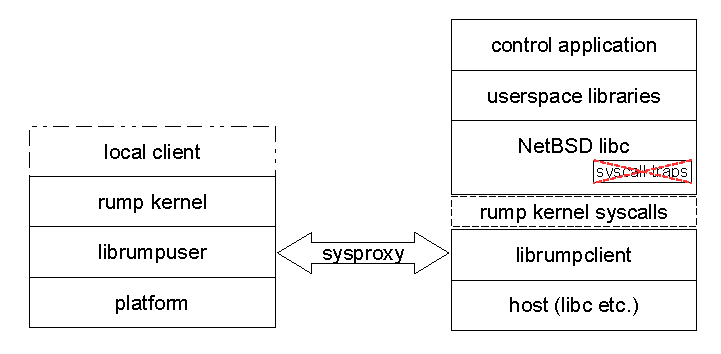
\includegraphics[width=\linewidth]{imgs/rumpctrl-stack}
\caption[Architecture of rumpctrl]{\textbf{Architecture of rumpctrl}.
The stack on the left is the rump kernel stack being controlled.
That stack may or may not include a local client.  For example,
a Rumprun unikernel instance is likely to include a local client, while
\texttt{\detokenize{rump_server}} (Section~\ref{sect:rumpserver}) will
not.  The stack on the right runs in POSIX userspace, and communicates
with the rump kernel over a sysproxy transport.
}
\label{fig:rumpctrl-stack}
\end{figure}

The usage of rumpctrl follows the same principles as remote clients
(Section~\ref{sect:remoteclient}); the environment variable
\verb+RUMP_SERVER+ contains the URL which points the client to the
server.  Additionally, rumpctrl provides a source'able script which sets
the rumpctrl commands at the front of \verb+PATH+.
In the following demonstration we have a rump
kernel server (in this case a Rumprun unikernel) listening
to sysproxy commands on a management interface at 10.0.0.2:12345.
Additionally, we demonstrate the \verb+rumpctrl_listcmds+ command,
which prints the commands provided by rumpctrl.

{\scriptsize
\begin{verbatim}
$ . rumpctrl.sh
rumpctrl (NULL)$ sysctl hw.model
error: RUMP_SERVER not set
rumpclient init failed
rumpctrl (NULL)$ export RUMP_SERVER=tcp://10.0.0.2:12345
rumpctrl (tcp://10.0.0.2:12345)$ sysctl hw.model
hw.model = rumpcore (virtual)
rumpctrl (tcp://10.0.0.2:12345)$ rumpctrl_listcmds
arp             ed              mkdir           newfs_ext2fs    rndctl
cat             fsck            mknod           newfs_msdos     route
cgdconfig       fsck_ext2fs     modstat         npfctl          rtadvd
chmod           fsck_ffs        mount           pax             sysctl
chown           fsck_msdos      mount_ext2fs    pcictl          umount
cp              halt            mount_ffs       ping            vnconfig
dd              ifconfig        mount_msdos     ping6           wlanctl
df              ktrace          mount_tmpfs     raidctl         wpa_passphrase
disklabel       ln              mv              reboot          wpa_supplicant
dump            ls              ndp             rm
dumpfs          mixerctl        newfs           rmdir
\end{verbatim}}

\subsection{fs-utils}
\label{sect:fs-utils}

Fs-utils~\cite{ysmal:fs-utils} (\url{http://repo.rumpkernel.org/fs-utils})
is a suite of userspace file system utilities (hence the name) which
intrinsically contain file system drivers; the utilities
do not use file system drivers from the host kernel.  The motivations
for building such a suite are the usual: running the file system driver
in userspace does only not depend on having support in the host kernel,
but also does not risk a host kernel compromise in case of a corrupt or
maliciously corrupted file system image.  In the permissions department,
read and optionally write permissions to the image are enough, no elevated
permissions are needed by the user running the utilities.

The implementation of fs-utils consists of standard standard NetBSD file
utilities (\texttt{ls}, \texttt{cat}, \texttt{mv}, etc.) which use rump
kernel file system drivers as local clients.  Doing so preserves the
normal usage of the utilities, \eg \texttt{ls} accepts the familiar
\texttt{-ABcFhL} parameter string.

The only exception to command line arguments is that the first parameter
is interpreted as the location specifier the file system is mounted from.
The tools make an attempt to auto-detect the type of file system, so passing the file system
type is optional.  For example, \verb+fsu_ls /dev/rwd0a -l+ might list
the contents of
a FFS on the hard drive, while \verb+fsu_ls 10.181.181.181:/m/dm -l+
would do the same for an NFS
export~\footnote
{
	In case of NFS, the \textit{sockin} networking facility
	(Section~\ref{sect:networking}) is used, so no TCP/IP stack
	configuration is required.
}.

Alternative ways of implementing such a file system utility suite are
to write or port the file system drivers, or use full operating systems in
virtual machines.  Those approaches are demanding in terms of programming
work or runtime resources, respectively.


\subsection{Summary}

In this chapter we examined the ecosystem of tools and products built on
top of rump kernels.  At the center of the ecosystem is the
\texttt{buildrump.sh}
script, which allows building rump kernels on any POSIX-like system for
a variety of targets.  We discussed examples of what to build on top.
One example was the Rumprun unikernel, which allows running POSIX'y
applications on bare metal and the cloud.  Another example was the
fs-utils tool suite, which consists of tools capable of accessing and
modifying file system images.
